\documentclass[10pt]{article}
\usepackage[usenames]{color} %used for font color
\usepackage{amssymb} %maths
\usepackage{amsmath} %maths
\usepackage[utf8]{inputenc} %useful to type directly diacritic characters
\usepackage[letterpaper, portrait, margin=1.5in]{geometry}
\usepackage{multicol}
\usepackage{graphicx,wrapfig}
\usepackage{hyperref}
\begin{document}
\subsection*{MSDS600 Week 6 Assignment - Nathan Worsham}
\subsection*{Recreate the R part of this experiment using your computer.}  
Following the instructions provided I ran the following: 
\begin{verbatim}
library(e1071) 
setwd("/Users/worshamn/Dropbox/Documents/Regis/MSDS600/week6/") 
srd1 <- read.csv("srd1.csv",header=FALSE) 
srd2 <- read.csv("srd2.csv",header=FALSE) 
y1 <- rep(0,1000) 
y2 <- rep(1,1000) 
y <- factor(c(y1,y2)) 
x <- rbind(srd1,srd2) 
model <- svm(x,y,type="C-classification") 
p <- predict(model,x) 
plot(array(p)) 
\end{verbatim}
I received a similar looking plot that the assignment showed: 
\begin{figure}[!h]
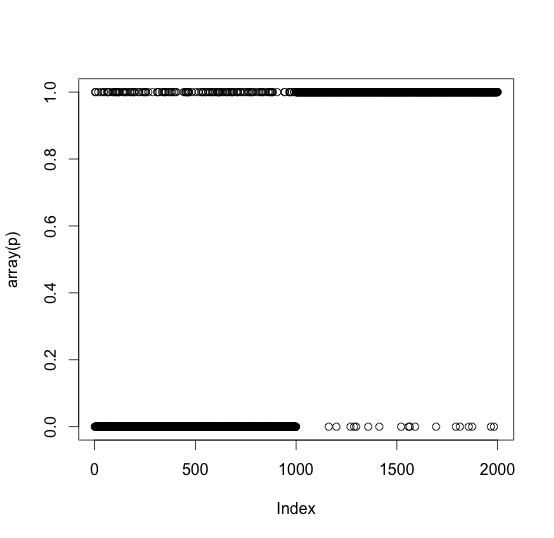
\includegraphics[scale=0.37]{Rplot_sd1v2.png}
\centering
\end{figure}
\subsection*{See if you can find other ways to display the predictions.} 
Looking for other “ways” to display the predictions, I went back to what I stumbled upon last week which turns out to also be in the reading for this week which is the confusion matrix and the accuracy check:\pagebreak 
\begin{verbatim}
> conf.mat <- table("Predictions" = p, Actual = y) 
> print(conf.mat) 
           Actual 
Predictions   0   1 
          0 865  18 
          1 135 982 
> (accuracy <- sum(diag(conf.mat)) / length(y) * 100) 
[1] 92.35 
\end{verbatim}
Maybe this is not a visualization per se, but I also tried experimenting around with other visualizations. From class discussions about functions, \verb|cloud| and \verb|scatterplot3d| I found neither to show any useful way of showing this data. I also recreated the original scatterplot in the assignment: 
\begin{verbatim}
ggplot() +  
  geom_point(data=srd1, aes(x=V1,y=V2), color = 'blue', size=1) +  
  geom_point(data=srd2, aes(x=V1,y=V2), color = 'red', size=1) 
\end{verbatim}
Then I tried adding the prediction data on top: 
\begin{verbatim}
library(ggplot2) 
library(Rmisc) 
df=data.frame(x,y=as.numeric(as.character(y))) 
df.0 <- df[df$y==0,] 
df.1 <- df[df$y==1,] 
ggplot() +  
  geom_point(data=srd1, aes(x=V1,y=V2), color = 'blue', size=1) +  
  geom_point(data=srd2, aes(x=V1,y=V2), color = 'red', size=1) + 
  geom_point(data=df.0, aes(x=V1,y=V2), color = 'orange', size=1) +  
  geom_point(data=df.1, aes(x=V1,y=V2), color = 'green', size=1) 
\end{verbatim}
After doing this all I could see was the last 2 plots, so plotting the 2 plots side by side: 
\begin{figure}[!h]
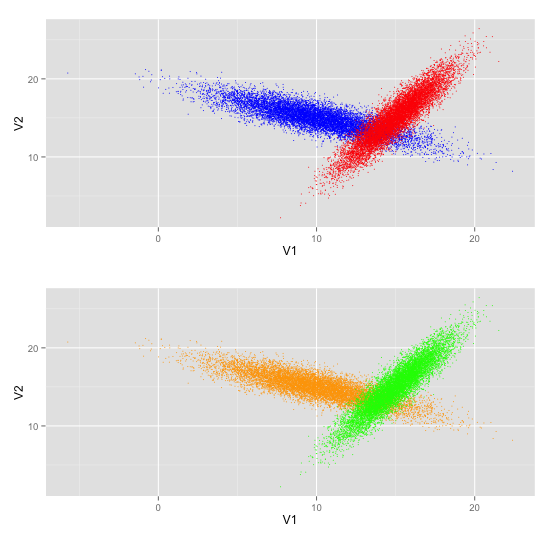
\includegraphics[scale=0.37]{rdVsPred.png}
\centering
\end{figure}\\*
\newpage\
\\* I see that the two plots look pretty much the same. I then stumbled upon receiver operating characteristic, or ROC curves. A ROC curve is essentially a way to plot the confusion matrix in terms of “true positive rate” against “false positive rate” and the closer the curve is to the upper left corner the more accurate it is (UNMC.edu, n.d.).  
\begin{verbatim}
library(ROCR) 
p <- predict(model,x, type='decision') 
roc.curve1 <- performance( prediction(as.numeric(as.character(p))
  ,as.numeric(as.character(y))),measure='tpr', x.measure='fpr' ) 
plot(roc.curve1) 
\end{verbatim}
\begin{figure}[!h]
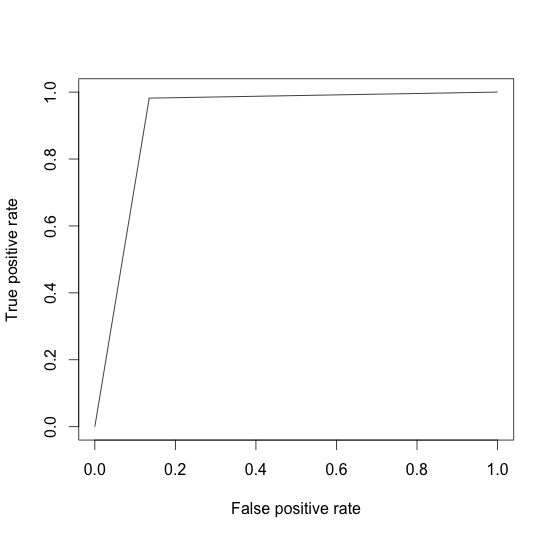
\includegraphics[scale=0.37]{sd_roc.png}
\centering
\end{figure}

After all of this I conclude that the confusion matrix and accuracy is the best way to see how this prediction performed which is what the ROC curve shows but I find summing this up to one number (accuracy) is more valuable as a quick measurement to know if your model is predicting better rather than looking at a graph for the same data.  
\subsection*{Train the svm model using the 1000 length data and then predict the 10,000 length data.  Compare the predictions with the data.  See the ideas of cross validation.} 
Adding in the rd1 and rd2 as the prediction data this time: 
\begin{verbatim}
library(e1071) 
setwd("/Users/worshamn/Dropbox/Documents/Regis/MSDS600/week6/") 
srd1 <- read.csv("srd1.csv",header=FALSE) 
srd2 <- read.csv("srd2.csv",header=FALSE) 
rd1 <- read.csv("rd1.csv",header=FALSE) 
rd2 <- read.csv("rd2.csv",header=FALSE) 
y1 <- rep(0,1000) 
y2 <- rep(1,1000) 
a1 <- rep(0,10000) 
a2 <- rep(1,10000) 
y <- factor(c(y1,y2)) 
a <- factor(c(a1,a2)) 
x <- rbind(srd1,srd2) 
z <- rbind(rd1,rd2) 
model <- svm(x,y,type="C-classification") 
p <- predict(model,z) 
plot(array(p)) 
conf.mat <- table("Predictions" = p, Actual = a) 
print(conf.mat) 
(accuracy <- sum(diag(conf.mat)) / length(a) * 100) 

> print(conf.mat) 
           Actual 
Predictions    0    1 
          0 8595  150 
          1 1405 9850 
> (accuracy <- sum(diag(conf.mat)) / length(a) * 100) 
[1] 92.225 
\end{verbatim}
The accuracy is similar at 92.225\% when it predicted against the srd data but plotting the data as I did previously in the exercise makes the 1 values almost look like a solid line because there are so many false positives (1405). Now looking into cross-validation which is "primarily a way of measuring the predictive performance of a statistical model" (Hyndman, 2010). In its simplest form, using a testing and training set from the same data \textit{is} cross-validation and is called the holdout method (Schneider, 1997) which is something that I had (unknowingly) started doing last week. There is another type though called k-fold, where the data is broken into k subsets and the holdout method is repeated k times (Schneider, 1997). The SVM function has an option to do this by providing \verb|cross = k|, then running \verb|summary(model)| to see the results, it runs the k-fold cross-validation and takes the average of subset accuracies to give a overall accuracy. When I set \verb|cross| to 10, it tells me the accuracy is 92.05\% which is remarkably close to what I got when I ran the rd data set. \\*\\*
10-fold cross-validation on training data: 
\begin{verbatim}
Total Accuracy: 92.05  
Single Accuracies: 
 92 93 93.5 94 91.5 89 93.5 92.5 88 93.5  
\end{verbatim}
Consequently I tried \verb|cross| set to 5 and got 91.8\% accuracy, 20 received 91.95\% accuracy, and 8 produced 92.1\%. In the video “An Introduction To Cross-Validation” on Salford Systems website, they talk about this phenomenon that usually around 10 is the better k value. Using k-fold cross-validation is important because we want to have an idea before relying on a model of how accurate it will be against data that it has not yet seen which really is the whole point of machine learning—if the model cannot accurately predict the values, then we cannot trust the model.  
\subsection*{Is there anyway to remove the ambiguity between the two classes given the existing data?  What about if you could add additional measurements for each data point?}
It would seem that only having 2 data points to try to differentiate the two classes that overlap is not sufficient enough to remove the ambiguity between them. As Hashemi (n.d.) points out “ambiguous data do not show any inconsistency with the other datapoints in the sameclass. Thus, techniques like residual analysis and different distance measures like Cook’s distance cannot distinguish them.” I find it even easier to understand when Hashemi says “because data points in (the overlapping) region have equal probability to belong to either of the two classes”. I did find in SVM that tuning some of the additional arguments can change how accurate the model is and in some cases improve on it very slightly, though much of it I have trouble understanding what it is or how it works. The first change was cost. Moving this value down below 1, decreased the accuracy while increasing it increases accuracy slightly. I found that cost=100 improved the model from 92.225\% to 92.88\%: 
\begin{verbatim}
> model <- svm(x,y,type="C-classification",cross=10,cost=100) 
> p <- predict(model,z) 
> conf.mat <- table("Predictions" = p, Actual = a) 
> print(conf.mat) 
           Actual 
Predictions    0    1 
          0 8898  322 
          1 1102 9678 
> (accuracy <- sum(diag(conf.mat)) / sum(conf.mat) * 100) 
[1] 92.88 
\end{verbatim}
While moving it to 1000 or higher resulted in lower than 92.88\% accuracy. Trying to figure out what exactly cost is, the help file lists it as “cost of constraints violation”. According to Hilary (2015), cost or C is a regularization parameter and large C makes constraints harder to ignore. I also tried setting the kernel to all of the different options, no matter what cost was set to I was getting lower accuracy. I found that increasing the tolerance with the cost set to 100 also improved the accuracy (92.935\%). I found that applying weighted values to y (normally each value 0 or 1 is worth the same) also can improve the accuracy but only at seemingly strange weighted values. When I weighted 0 as 1.21 and 1 as 0.89, I finally broke through the 93\% barrier with an accuracy of 93.04\%: 
\begin{verbatim}
> wts <- table(y) 
> wts[1] <- 1.21 
> wts[2] <- 0.89 
> model <- svm(x,y,type="C-classification",cross=10,cost=100,tolerance=1
  ,class.weights=wts,gamma=0.5) 
> p <- predict(model,z) 
> conf.mat <- table("Predictions" = p, Actual = a) 
> print(conf.mat) 
           Actual 
Predictions    0    1 
          0 8980  372 
          1 1020 9628 
> (accuracy <- sum(diag(conf.mat)) / sum(conf.mat) * 100) 
[1] 93.04 
\end{verbatim}
During my research, I found that this seems to be called “Non linearly separable data” and there possibly exist ways to separate the data by adding a z dimension (height) but essentially I ran myself empty trying to figure it out. However I did find there is a function in the e1071 package called “tune” which can try to help find the best parameters. I experimented with this package for awhile but was never able to beat my own findings, though it was very close. 

\subsection*{Reference}
Hyndman, Rob J, 2010. Retrieved from \href{url}{http://robjhyndman.com/hyndsight/crossvalidation/}\\*\\*
UNMC.edu, n.d. Retrieved from \href{url}{http://gim.unmc.edu/dxtests/roc2.htm|}\\*\\*
Schneider, Jeff, 1997. Retrieved from \href{url}{https://www.cs.cmu.edu/~schneide/tut5/node42.html}\\*\\*
Salford Systems, n.d. An Introduction To Cross-Validation. Retrieved from\\*
\href{url}{http://www.salford-systems.com/videos/tutorials/how-to/an-introduction-to-cross-validation}\\*\\*
Hilary, 2015. Lecture 2: The SVM classifier.\\*
Retrieved from \href{url}{http://www.robots.ox.ac.uk/~az/lectures/ml/lect2.pdf}

\end{document}